\documentclass[tikz]{standalone}
\usepackage{tikz}
\usepackage{amssymb}
\usetikzlibrary{positioning}
\usetikzlibrary{calc}
\usetikzlibrary{arrows,shapes,snakes,automata,petri}
\begin{document}
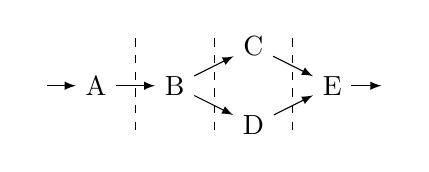
\begin{tikzpicture}
\node[](startA) at (-0.75,0){};
\node[](A) at (0,0){A};
\node[](B) at (1,0){B};
\node[](C) at (2,0.5){C};
\node[](D) at (2,-0.5){D};
\node[](E) at (3,0){E};
\node[](endE) at (3.75,0){};

\draw[dashed](0.5,0.6)--(0.5,-0.6);
\draw[dashed](1.5,0.6)--(1.5,-0.6);
\draw[dashed](2.5,0.6)--(2.5,-0.6);

\path
(startA) edge[-latex]node{} (A)
(A) edge[-latex]node{} (B)
(B) edge[-latex]node{} (C)
(B) edge[-latex]node{} (D)
(D) edge[-latex]node{} (E)
(C) edge[-latex]node{} (E)
(E) edge[-latex]node{} (endE);
\end{tikzpicture}
\end{document}